\subsection{视图}\label{subsec:czjh2-8-1}

\begin{wrapfigure}[7]{r}{5cm}
    \centering
    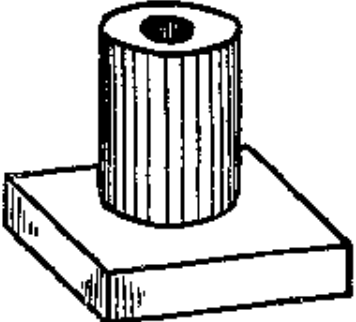
\includegraphics[width=3cm]{../pic/czjh2-ch8-01.png}
    \caption{}\label{fig:czjh2-8-1}
\end{wrapfigure}

图 \ref{fig:czjh2-8-1} 是工厂里常见的一个机械零件的直观图,这种图虽富有立体感,
但不能准确地表示出物体各部分的真实形状和内部结构。
如长方形变成了平行四边形,圆变成了椭圆,并且看不清圆孔的深度,图形各部分尺寸也有了变化。
因此,一般不根据直观图来加工零件,而把它作为辅助图来使用。

为了准确地表示物体的实际形状和尺寸大小,在生产中主要采用视图,视图是用投影原理画出来的。

\subsubsection{投影}

投影现象广泛地存在于自然界和日常生活中,如在灯光下,将两手交叉握紧,
墙上就会出现象动物头部的影子(图 \ref{fig:czjh2-8-2}),墙壁是投影面,光线是投射线,
影子就是手在墙上的投影,由于灯光的光线可以看作是从一点发出的,
我们称这种投影为\zhongdian{中心投影}。

又如在阳光下,树的影子是树在地面上的投影,地面是投影面,光线是投射线。
由于太阳的光线可看作是平行的,这时,我们称这种投影为\zhongdian{平行投影}。

\begin{figure}[htbp]
    \centering
    \begin{minipage}[b]{7cm}
        \centering
        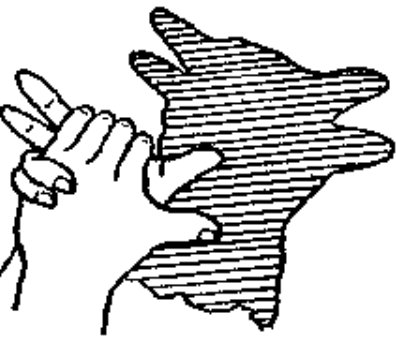
\includegraphics[width=4cm]{../pic/czjh2-ch8-02.png}
        \caption{}\label{fig:czjh2-8-2}
    \end{minipage}
    \begin{minipage}[b]{7cm}
        \centering
        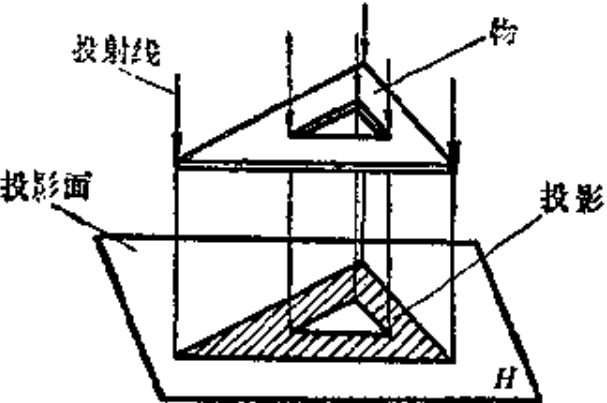
\includegraphics[width=6cm]{../pic/czjh2-ch8-03.png}
        \caption{}\label{fig:czjh2-8-3}
    \end{minipage}
\end{figure}

在平行投影中,如果投射线垂直于投影面,那么这种投影就称为\zhongdian{正投影}。
如图 \ref{fig:czjh2-8-3},一块三角板对于投影面 $H$ 平放着,光线垂直于投影面,
这时三角板的投影与它本身的形状、大小都一样。

我们看出,正投影能够反映物体的真实形状和大小。
因此,在工程技术上使用的图纸,多采用正投影方法绘制。


\subsubsection{正投影的规律}

(1)线段的正投影

如图 \ref{fig:czjh2-8-4},
点 $A$ 的投影为点 $A'$,记作 $A \to A'$,
点 $B$ 的投影为点 $B'$,记作 $B \to B'$;
线段 $AB$ 的投影为线段 $A'B'$,记作 $AB \to A'B'$。

\begin{figure}[htbp]
    \centering
    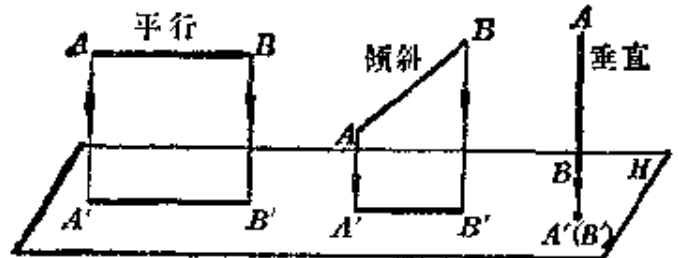
\includegraphics[width=8cm]{../pic/czjh2-ch8-04.png}
    \caption{}\label{fig:czjh2-8-4}
\end{figure}

当 $AB$ 平行于投影面 $H$ 时,$A'B' = AB$,“长不变”;

当 $AB$ 倾斜于投影面 $H$ 时,$A'B' < AB$,“长缩短”;

当 $AB$ 垂直于投影面 $H$ 时,$A' \equiv B'$\footnotemark,“成一点”。
\footnotetext{$A' \equiv B'$ 表示点 $A'$、$B'$ 重合,“$\equiv$” 在这里是重合记号。}

由此得到线段的正投影规律:

\begin{center}
    \framebox{\zhongdian{平行长不变,倾斜长缩短,垂直成一点。}}
\end{center}


(2)平面形的正投影

如图 \ref{fig:czjh2-8-5},平面形 $P$ (即四边形 $ABCD$)在投影面 $H$ 上的投影为四边形 $A'B'C'D'$。

\begin{figure}[htbp]
    \centering
    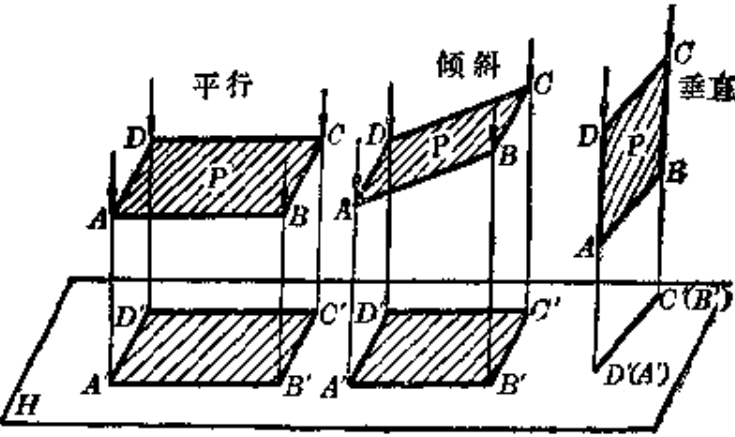
\includegraphics[width=8cm]{../pic/czjh2-ch8-05.png}
    \caption{}\label{fig:czjh2-8-5}
\end{figure}

$\because$ \quad $AB \to A'B'$, $BC \to B'C'$, $CD \to C'D'$, $DA \to D'A'$,

$\therefore$ \quad $\text{四边形} \; ABCD \to \text{四边形} \; A'B'C'D'$。

当图形 $P$ 平行于投影面 $H$ 时,$\text{四边形} \; ABCD \quandeng \text{四边形} \; A'B'C'D'$,“形状不变”;

当图形 $P$ 倾斜于投影面 $H$ 时,“形状改变”;

当图形 $P$ 垂直于投影面 $H$ 时,“成线段”。

由此得到平面形的正投影规律:

\begin{center}
    \framebox{\zhongdian{平行形不变,倾斜形改变,垂直成线段。}}
\end{center}


(3)几何体的正投影

一个正方体与投影面 $V$ 的相对位置如图 \ref{fig:czjh2-8-6} 所示,正方体有六个面:
面 $P$、$Q$、$R$ 和分别与它们相对的三个面。
根据平面形的正投影规律,我们可以得到这六个面的正投影。

因为面 $P$、$Q$ 及其相对的面都与投影面 $V$ 垂直,就有

面 $P \to A'B'$,面 $P$ 相对的面 $\to D'C'$;

面 $Q \to B'C'$,面 $Q$ 相对的面 $\to A'D'$;

面 $R$ 及其相对的面平行于投影面 $V$,就有

面 $R \to$ 正方形 $A'B'C'D'$,面 $R$ 相对的面 $\to$ 正方形 $A'B'C'D'$。

所以,正方体在投影面 $V$ 上的正投影是正方形 $A'B'C'D'$。

物体的正投影称为物体的\zhongdian{视图}。

物体的视图与物体对于投影面的位置有关,当正方体在如图 \ref{fig:czjh2-8-6} 中的位置吋,
它在投影面 $V$ 上的视图是一个正方形。而在其他位置时就不一定是正方形。


\begin{figure}[htbp]
    \centering
    \begin{minipage}[b]{7cm}
        \centering
        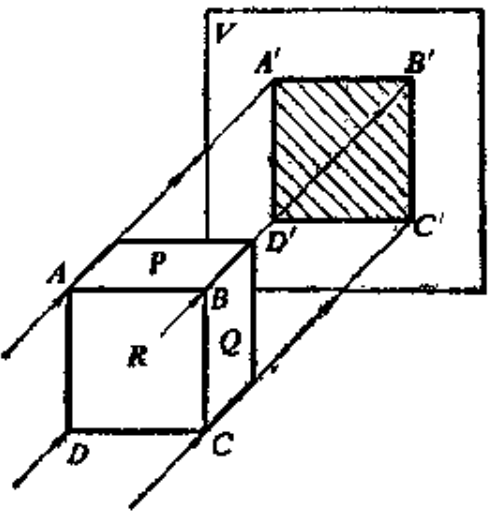
\includegraphics[width=5cm]{../pic/czjh2-ch8-06.png}
        \caption{}\label{fig:czjh2-8-6}
    \end{minipage}
    \begin{minipage}[b]{7cm}
        \centering
        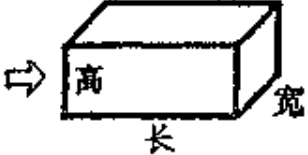
\includegraphics[width=4cm]{../pic/czjh2-ch8-subsec1-lx-03.png}
        \caption*{(第 3 题)}
    \end{minipage}
\end{figure}


\begin{lianxi}

\xiaoti{举出几个日常生活中的例子说明投影概念。}

\xiaoti{有一圆形木板,它的正投影一定是圆形吗?为什么?}

\xiaoti{已知长方体的长、宽、高分别为 3 cm、2 cm、1 cm,
    说出图中所示方向的视图,并用平面形的正投影规律加以说明。
}

\end{lianxi}

